\subsect{Sprint 10}{sprint10}

\underline{Fecha de inicio}: 11/03/2023

\underline{Fecha de fin}: 11/04/2023

\underline{Objetivo}:
Migración del filtro de imágenes NSFW a Python y bloqueo de usuarios.

\underline{Descripción}:
La integración del modelo de inteligencia artificial con JavaScript no ha funcionado como se esperaba, por lo que se
ha decidido migrar el código a Python, que es el lenguaje en el que se ha desarrollado el modelo.\ Esto ofrece
una mejora de rendimiento a la hora de procesar las imágenes que no se puede conseguir con JavaScript.\ Además, se
ha implementado un sistema de bloqueo de usuarios para evitar que envíen más de 5 imágenes inapropiadas.\ En caso de
que lo hagan, se les bloqueará la cuenta durante 24 horas.

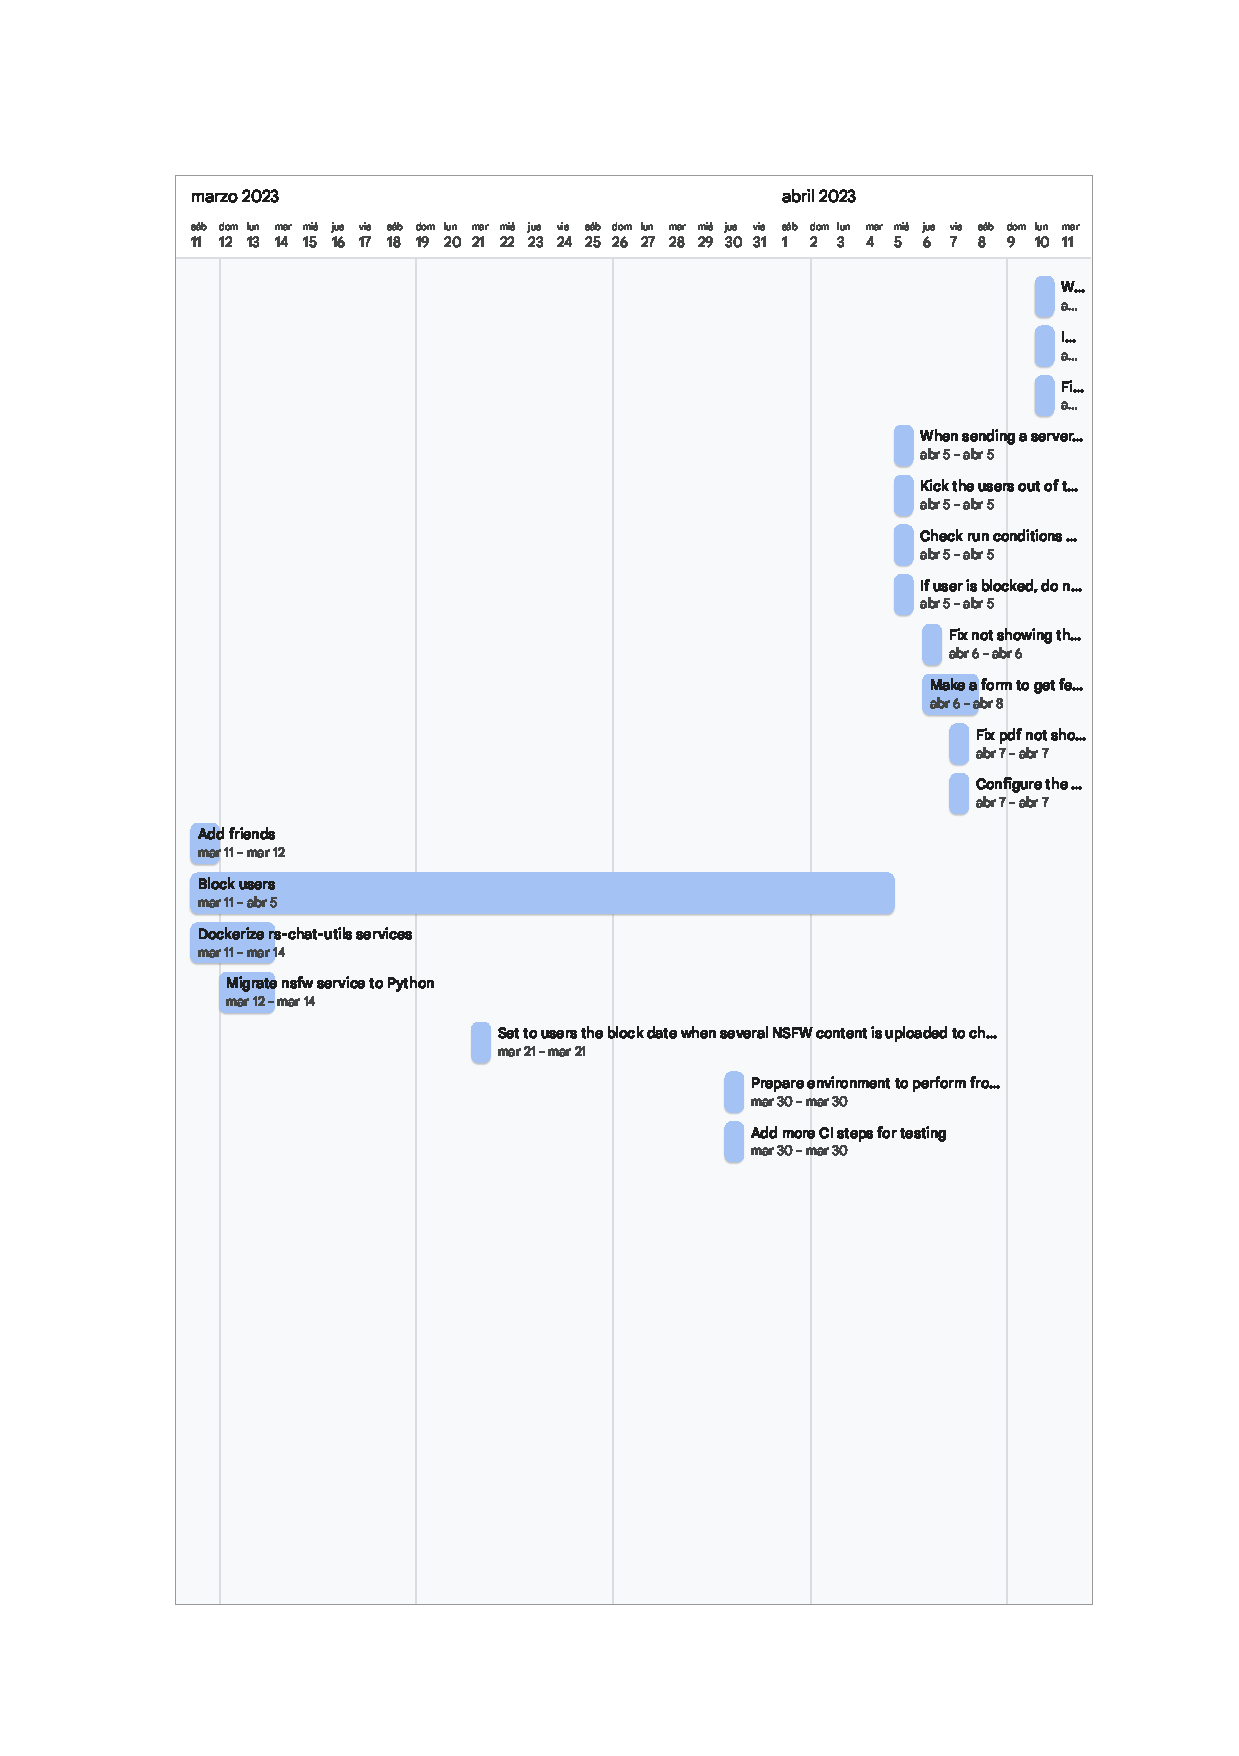
\includepdf[pages=-]{backlog/sprints/Sprint10.pdf}
